\documentclass[../main.tex]{subfiles}
\begin{document}

\begin{figure}[H]
\centering
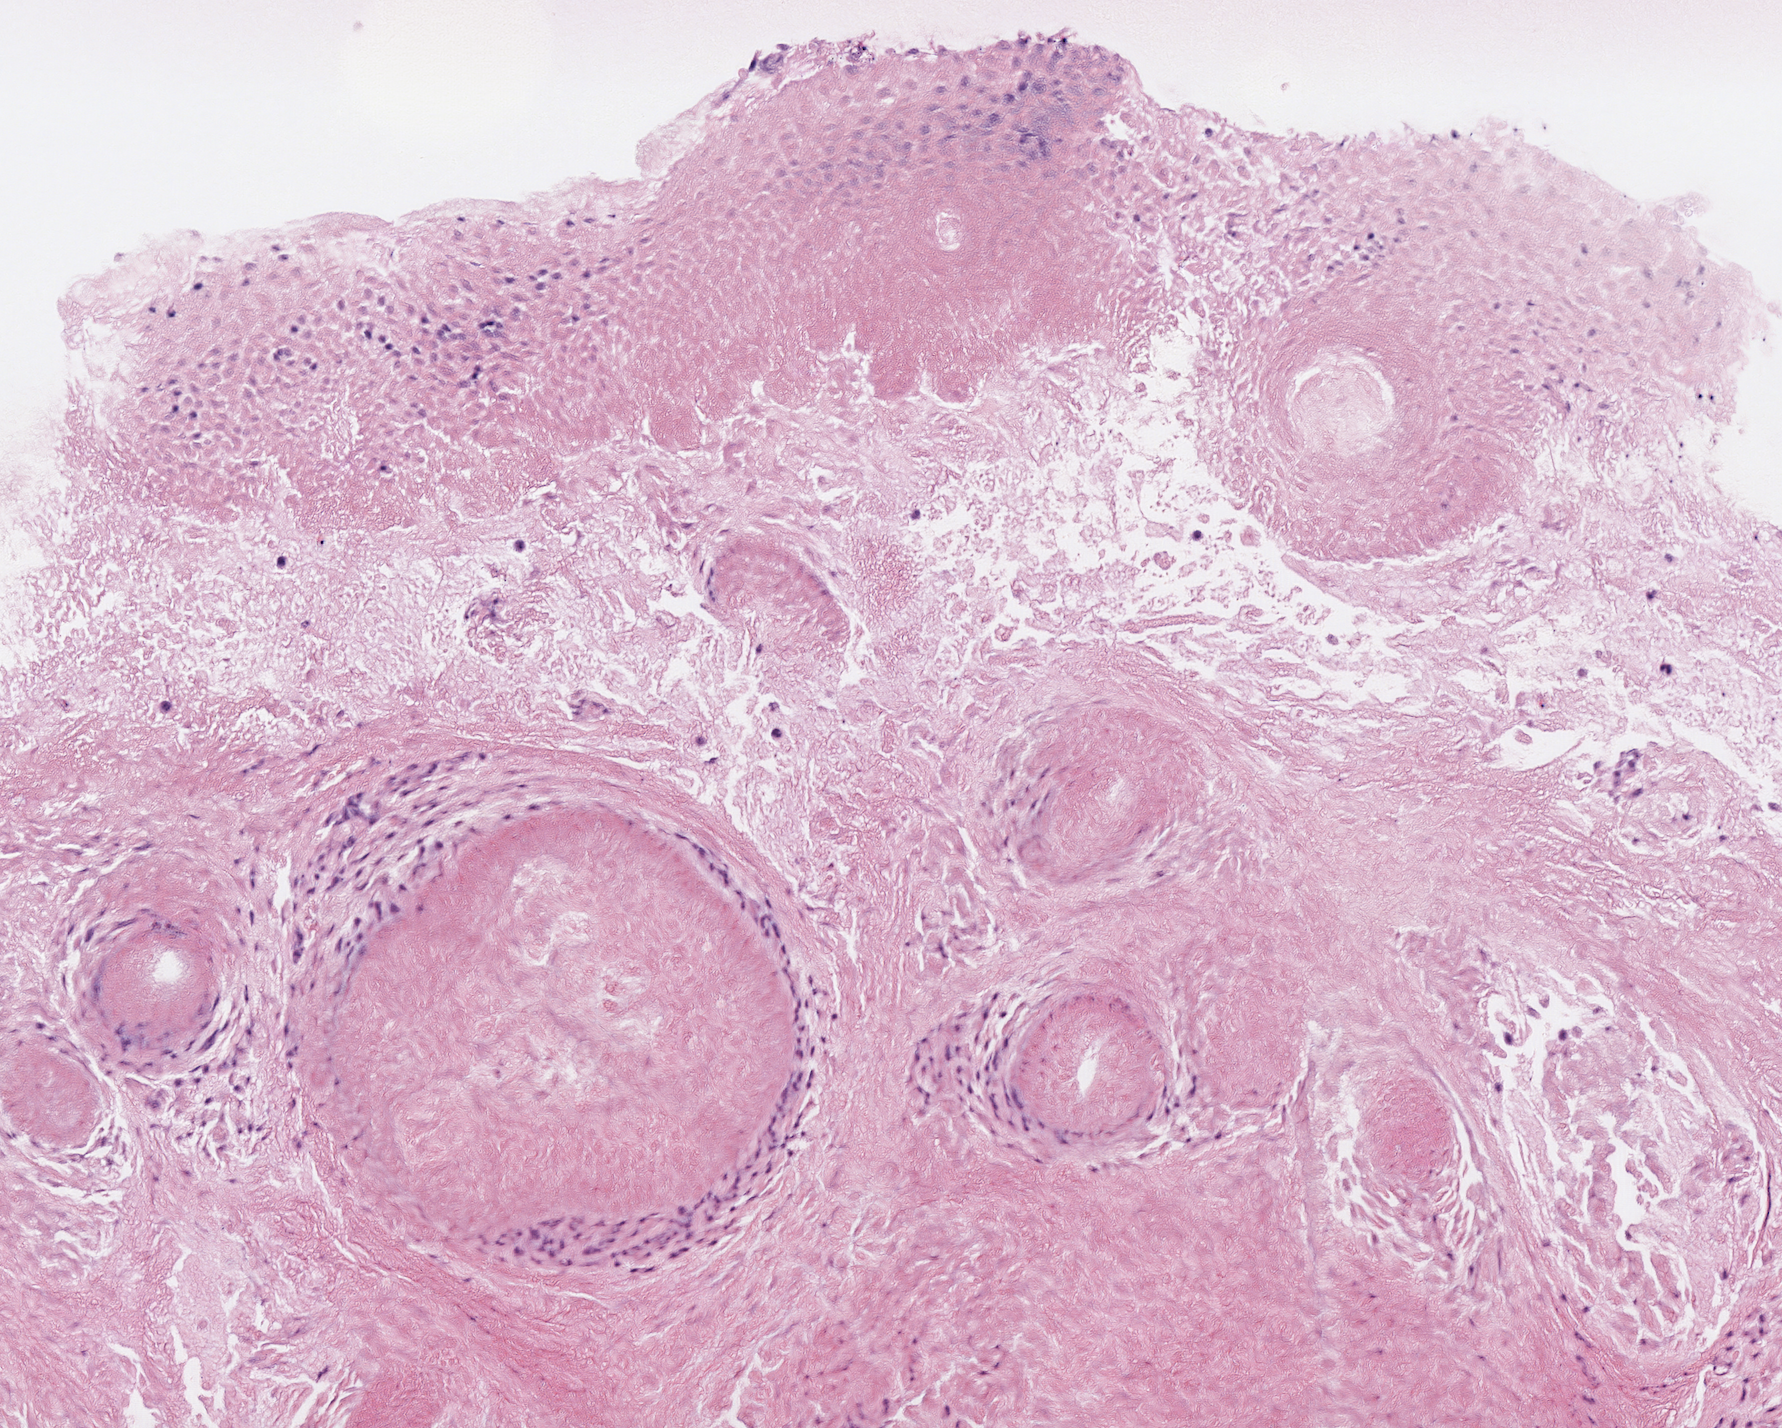
\includegraphics[width=0.9\linewidth]{DetailFigure2}
\caption{``No se observan los núcleos de la epidermis ni de los folículos.
Tampoco la imagen del tumor en la parte inferior de la misma (BCC).''}
\end{figure}

\begin{figure}
\centering
\includegraphics[width=0.9\linewidth]{DetailFigure3}
\caption{``Al tratarse de otro tumor (SCC), también es fundamental observar los
núcleos de las perlas de queratina, que es lo que lo diferencia de otro tipo
de tumores.''}
\end{figure}

\end{document}
